% Source: ml_gradient_misconception.tex
\begin{notechapter}
\chapter{The Gradient in Machine Learning}\label{ch:gradient-misconception}
\chaptersubtitle{Why common visualizations are misleading}

\section{Introduction}

There is a widespread misconception in machine learning courses about what
the gradient represents geometrically.

\begin{warning}[Common Mistake in ML Courses]
Many visualizations show the gradient as a vector "tangent to the loss surface"
or "sliding down a slope." 

\textbf{This is geometrically incorrect!}
\end{warning}

Let me explain what's actually happening.

\section{The Setup in Machine Learning}

\subsection{The Loss Function}

In machine learning, we have:
\begin{itemize}
    \item \textbf{Parameters:} $\theta \in \mathbb{R}^n$ (e.g., weights and biases of a neural network)
    \item \textbf{Loss function:} $L : \mathbb{R}^n \to \mathbb{R}$ (measures prediction error)
    \item \textbf{Goal:} Minimize $L(\theta)$
\end{itemize}

\textbf{Example:} For a neural network with 1000 parameters, $\theta \in \mathbb{R}^{1000}$.

\subsection{Gradient Descent}

The update rule is:
\[
\theta_{k+1} = \theta_k - \alpha \nabla L(\theta_k)
\]

where:
\begin{itemize}
    \item $\theta_k \in \mathbb{R}^n$ is the current parameter vector
    \item $\nabla L(\theta_k) \in \mathbb{R}^n$ is the gradient
    \item $\alpha > 0$ is the learning rate
\end{itemize}

\section{What the Gradient Actually Is}

\subsection{The Gradient Lives in Parameter Space}

\begin{definition}[The Gradient]
The gradient $\nabla L(\theta) \in \mathbb{R}^n$ is a vector in \textbf{parameter space}, not in the space where the loss surface lives.
\end{definition}

\textbf{Key facts:}
\begin{itemize}
    \item $\nabla L(\theta) \in \mathbb{R}^n$ (same dimension as $\theta$)
    \item It points in the direction of \textbf{steepest ascent} of $L$ in parameter space
    \item It is \textbf{orthogonal} to level sets $\{"\theta : L(\theta) = c\}$ in parameter space
    \item It has \textbf{nothing to do} with tangent vectors to the graph of $L$
\end{itemize}

\subsection{Level Sets in Parameter Space}

The level sets of $L$ are:
\[
\{\theta \in \mathbb{R}^n : L(\theta) = c\}
\]

These are $(n-1)$-dimensional surfaces in $\mathbb{R}^n$ (parameter space).

\textbf{The gradient is perpendicular to these level sets!}

\begin{center}
\begin{tikzpicture}[scale=2]
    % Draw parameter space (2D for visualization)
    \draw[->] (-0.5,0) -- (2.5,0) node[right] {$\theta_1$};
    \draw[->] (0,-0.5) -- (0,2.5) node[above] {$\theta_2$};
    
    % Draw level curves (ellipses)
    \draw[blue, thick] (1,1) ellipse (0.3 and 0.5);
    \draw[blue, thick] (1,1) ellipse (0.6 and 1.0);
    \draw[blue, thick] (1,1) ellipse (0.9 and 1.5);
    
    \node[blue] at (1.2, 1.6) {$L = c_1$};
    \node[blue] at (1.2, 2.1) {$L = c_2$};
    
    % Point in parameter space
    \coordinate (theta) at (1.67, 2);
    \fill[red] (theta) circle (1pt) node[below left] {$\mathbf{\theta}_k$};
    
    % Gradient (perpendicular to level curve, pointing outward)
    \draw[red, very thick, ->] (theta) -- ++(0.4, 0.23) node[right] {$\nabla L(\theta_k)$};
    
    % Tangent to level curve
    \draw[green!60!black, thick] ($(theta) + (-0.14, 0.3)$) -- ($(theta) + (0.17, -0.3)$);
    \node[green!60!black] at ($(theta) + (1.0, -0.4)$) {tangent to level set};
    
    % Show gradient is perpendicular
    \draw[dashed, gray] (theta) -- ++(0.5, -0.3);
    
    \node at (1.2, -0.8) {\textbf{Parameter Space } $\mathbb{R}^n$};
    \node[red] at (1.2, -1.1) {Gradient $\perp$ level curves};
\end{tikzpicture}
\end{center}

\section{The Misleading Visualization}

\subsection{What ML Courses Often Show}

Many courses show something like this:

\begin{center}
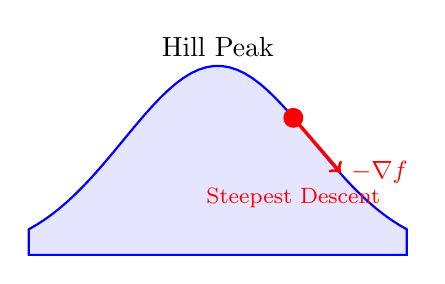
\begin{tikzpicture}[scale=1.2]
    % Draw the hill (Gaussian curve)
    \draw[thick, blue, fill=blue!10] 
        plot[domain=-2:2, samples=50] (\x, {2*exp(-\x*\x/2)}) -- (2,0) -- (-2,0) -- cycle;
    
    % Define the position of the ball (e.g., at x = 0.8)
    % y = 2*exp(-0.8^2/2) approx 1.45
    \coordinate (ball) at (0.8, 1.45);
    
    % Draw the "Ball"
    \fill[red] (ball) circle (3pt);
    
    % Direction of steepest descent (Negative Gradient)
    % The derivative of 2e^(-x^2/2) is -2x*e^(-x^2/2). 
    % At x=0.8, slope is approx -1.16.
    \draw[red, very thick, ->] (ball) -- ++(0.5, -0.58) 
        node[right, font=\small] {$-\nabla f$};
    
    % Labels
    \node[anchor=south] at (0,2) {Hill Peak};
    \node[red, font=\footnotesize] at (0.8, 0.6) {Steepest Descent};
\end{tikzpicture}
\end{center}

\textbf{The problem:} This suggests the gradient is a vector that "slides along" the loss surface, pointing "downhill."

\subsection{Why This is Wrong}

The graph of $L$ lives in $\mathbb{R}^{n+1}$ (parameter space + loss value):
\[
\text{Graph}(L) = \{(\theta, L(\theta)) : \theta \in \mathbb{R}^n\} \subseteq \mathbb{R}^{n+1}
\]

But the gradient $\nabla L(\theta) \in \mathbb{R}^n$ lives only in parameter space!

\textbf{These are different spaces!}

\section{What's Actually Happening}

\subsection{The Correct Picture}

Here's what gradient descent really does:

\begin{enumerate}
    \item We're at parameter vector $\theta_k \in \mathbb{R}^n$
    \item The gradient $\nabla L(\theta_k) \in \mathbb{R}^n$ points toward higher loss
    \item We move in the \textbf{opposite direction}: $\theta_{k+1} = \theta_k - \alpha \nabla L(\theta_k)$
    \item This is a movement \textbf{in parameter space}, not on the loss surface
\end{enumerate}

\begin{center}
\begin{tikzpicture}[scale=2.5]
    % Parameter space
    \draw[->] (-0.3,0) -- (2.5,0) node[right] {$\theta_1$};
    \draw[->] (0,-0.3) -- (0,2) node[above] {$\theta_2$};
    
    % Level sets
    \draw[blue, thick] (1.5, 0.8) ellipse (0.2 and 0.15);
    \draw[blue, thick] (1.5, 0.8) ellipse (0.4 and 0.3);
    \draw[blue, thick] (1.5, 0.8) ellipse (0.6 and 0.45);
    \draw[blue, thick] (1.5, 0.8) ellipse (0.8 and 0.6);
    
    \node[blue] at (2.35, 1.2) {level sets};
    
    % Minimum
    \fill[blue] (1.5, 0.8) circle (0.5pt) node[below right] {$\theta^*$ (minimum)};
    
    % Gradient descent trajectory
    \coordinate (t0) at (0.95, 1.6);
    \coordinate (t1) at (1.13, 1.31);
    \coordinate (t2) at (1.3, 1.05);
    \coordinate (t3) at (1.4, 0.9);
    
    \fill[red] (t0) circle (0.8pt) node[left] {$\theta_0$};
    \fill[red] (t1) circle (0.8pt) node[above left] {$\theta_1$};
    \fill[red] (t2) circle (0.8pt) node[above] {$\theta_2$};
    \fill[red] (t3) circle (0.8pt) node[right] {$\theta_3$};
    
    % Trajectory
    \draw[red, thick, ->] (t0) -- (t1);
    \draw[red, thick, ->] (t1) -- (t2);
    \draw[red, thick, ->] (t2) -- (t3);
    
    % Gradient at one point
    \draw[red, very thick, ->] (t0) -- ++(-0.27, 0.5) node[right] {$\nabla L(\theta_0)$};
    %\draw[red, dashed] (t0) -- ++(0.15, 0.19);
    
    % Perpendicular to level curve
    \draw[green!60!black, thick] ($(t0) + (-0.35, -0.15)$) -- ($(t0) + (0.7, 0.36)$);
    \node[green!60!black, rotate=27] at ($(t0) + (0.7, 0.27)$) {tangent to level set};
    
    \node[red] at (1.2, -0.5) {\textbf{Gradient descent in parameter space}};
\end{tikzpicture}
\end{center}

\subsection{Key Observations}

\begin{enumerate}
    \item \textbf{Movement is in parameter space} $\mathbb{R}^n$, not on the graph
    \item \textbf{Gradient points perpendicular to level sets}
    \item \textbf{We move opposite to the gradient} (toward lower loss)
    \item \textbf{Steps cross level sets perpendicularly} (when step size is small)
\end{enumerate}

\section{Why the Confusion?}

\subsection{The Visualization Problem}

When $n = 2$ (two parameters), we can visualize:
\begin{itemize}
    \item Parameter space as the $xy$-plane
    \item Loss function as height: $z = L(\theta_1, \theta_2)$
    \item This gives a 3D surface
\end{itemize}

\textbf{The trap:} We draw arrows on this 3D surface and call them "gradients."

But the gradient $\nabla L \in \mathbb{R}^2$ lives in the $xy$-plane, not on the 3D surface!

\subsection{What People Actually Mean}

When ML courses show an arrow "sliding down the surface," they're actually trying to show:

\begin{enumerate}
    \item The movement $\theta_k \to \theta_{k+1}$ projected onto the $xy$-plane
    \item Lifted to the graph to show the corresponding decrease in loss
\end{enumerate}

But this is \textbf{not} the gradient itself!

\section{The Correct Understanding}

\subsection{For $n = 2$ Parameters}

Let $L : \mathbb{R}^2 \to \mathbb{R}$ with $\theta = (\theta_1, \theta_2)$.

\textbf{Parameter space view:}
\begin{itemize}
    \item Look at the $\theta_1\theta_2$-plane from above
    \item Draw level curves $\{(\theta_1, \theta_2) : L(\theta_1, \theta_2) = c\}$
    \item The gradient $\nabla L(\theta) = \begin{bmatrix} \frac{\partial L}{\partial \theta_1} \\ \frac{\partial L}{\partial \theta_2} \end{bmatrix}$ is perpendicular to these curves
    \item This is a vector in the plane, pointing toward higher loss values
\end{itemize}

\textbf{3D surface view (for intuition):}
\begin{itemize}
    \item The graph is $\{(\theta_1, \theta_2, L(\theta_1, \theta_2))\} \subseteq \mathbb{R}^3$
    \item The tangent plane at a point has tangent vectors in $\mathbb{R}^3$
    \item These tangent vectors are \textbf{not} the gradient!
    \item The gradient is the projection of the "steepest ascent direction" onto the $\theta_1\theta_2$-plane
\end{itemize}

\subsection{For General $n$ Parameters}

When $n > 2$ (typical in ML: $n$ could be millions!):
\begin{itemize}
    \item Parameter space is $\mathbb{R}^n$
    \item Level sets are $(n-1)$-dimensional hypersurfaces
    \item Gradient $\nabla L(\theta) \in \mathbb{R}^n$ is perpendicular to these hypersurfaces
    \item We \textbf{cannot} visualize the graph (it's in $\mathbb{R}^{n+1}$)
    \item The only correct view is in parameter space
\end{itemize}

\section{The Geometric Truth}

\subsection{Relationship to the Graph}

If we \textit{must} relate the gradient to the graph, here's the correct statement:

\begin{theorem}[Gradient and Graph Tangent Space]
Let $L : \mathbb{R}^n \to \mathbb{R}$ and consider the graph:
\[
\Gamma = \{(\theta, L(\theta)) : \theta \in \mathbb{R}^n\} \subseteq \mathbb{R}^{n+1}
\]

At point $(\theta_0, L(\theta_0))$, tangent vectors to $\Gamma$ have the form:
\[
\begin{bmatrix} v \\ \nabla L(\theta_0)^\top v \end{bmatrix} \in \mathbb{R}^{n+1}
\]
where $v \in \mathbb{R}^n$ is arbitrary.

The gradient $\nabla L(\theta_0) \in \mathbb{R}^n$ is the \textbf{first $n$ components} of the "steepest ascent" tangent vector (when normalized appropriately). Precisely, projecting the vertical direction $e_{n+1}$ orthogonally onto the tangent space of $\Gamma$ (whose unit normal is $(-\nabla L, 1)/\sqrt{1 + \|\nabla L\|^2}$) gives the direction of steepest ascent of the height on the surface:
\[
\frac{1}{1 + \|\nabla L(\theta_0)\|^2}\begin{bmatrix} \nabla L(\theta_0) \\ \|\nabla L(\theta_0)\|^2 \end{bmatrix},
\]
whose first $n$ components are proportional to $\nabla L(\theta_0)$.
\end{theorem}

\textbf{But this is complicated and not how we should think about it!}

\subsection{The Right Mental Model}

\begin{center}
\fbox{\begin{minipage}{0.9\textwidth}
\textbf{Think of gradient descent as:}
\begin{enumerate}
    \item You're walking in parameter space $\mathbb{R}^n$
    \item At each point, you have a "height" value $L(\theta)$ (but you're not \textit{on} a height surface)
    \item The gradient tells you which direction in $\mathbb{R}^n$ increases height fastest
    \item You walk in the opposite direction
    \item As you walk, you cross level sets perpendicularly
\end{enumerate}
\end{minipage}}
\end{center}

\section{Why This Matters}

\subsection{Practical Implications}

Understanding the gradient correctly helps with:

\begin{enumerate}
    \item \textbf{Intuition about convergence:} Why gradient descent takes perpendicular steps to level sets
    
    \item \textbf{Understanding momentum:} Why momentum methods don't follow the gradient (they build velocity in parameter space)
    
    \item \textbf{Adaptive learning rates:} Methods like Adam adjust step sizes in different directions of parameter space
    
    \item \textbf{Second-order methods:} Newton's method uses curvature in parameter space, not on the loss surface
    
    \item \textbf{Manifold optimization:} When parameters live on manifolds (e.g., rotation matrices), we need to project gradients to tangent spaces
\end{enumerate}

\subsection{Common Questions Resolved}

\textbf{Q: "Why doesn't gradient descent always take the shortest path to the minimum?"}

\textbf{A:} Because the "shortest path" depends on the geometry of parameter space, while gradient descent follows a path perpendicular to level sets. These are different!

\textbf{Q: "Why do we need to normalize gradients in some applications?"}

\textbf{A:} The magnitude of $\nabla L$ tells us the \textit{rate} of change in parameter space. Normalizing makes all steps the same size in parameter space.

\section{The Correct Visualizations}

\subsection{For 2 Parameters (Correct)}

\textbf{Top-down view of parameter space:}
\begin{itemize}
    \item Draw contour lines (level sets)
    \item Show gradient vectors perpendicular to contours
    \item Show trajectory crossing contours
\end{itemize}

This is the correct mental model!

\subsection{For 3D (Use with Caution)}

If showing a 3D surface:
\begin{itemize}
    \item Make clear it's for visualization only
    \item Explicitly state that gradient lives in the base (parameter) space
    \item Show projections of vectors onto the base
    \item Avoid showing arrows "sliding along" the surface
\end{itemize}

\section{Summary}

\begin{enumerate}
    \item \textbf{Gradient $\nabla L(\theta)$ lives in parameter space
    $\mathbb{R}^n$}, not on the loss surface
    
    \item \textbf{The gradient is perpendicular to level sets}
    $\{\theta : L(\theta) = c\}$ in parameter space
    
    \item \textbf{The gradient is NOT tangent to the graph} of $L$
    
    \item \textbf{Gradient descent moves in parameter space}, stepping
    perpendicular to level sets
    
    \item \textbf{3D surface visualizations are misleading} because they suggest
    the gradient lives on the surface
    
    \item \textbf{The correct mental model:} Walking in parameter space,
    using gradients perpendicular to level sets

\end{enumerate}

The gradient is fundamentally a vector in parameter space that points perpendicular
to level sets. Everything else is just (potentially misleading) visualization for intuition.
\end{notechapter}
